
\documentclass[12pt,letterpaper]{article}
\usepackage[utf8]{inputenc}
\usepackage[spanish]{babel}
\usepackage{graphicx}
\usepackage[hidelinks]{hyperref}
\usepackage{hyperref}
\usepackage[left=2cm,right=2cm,top=2.5cm,bottom=2cm]{geometry}
\usepackage{graphicx} % figuras
\usepackage{float} % para usar [H]
\usepackage{amsmath}
\usepackage{stackrel} 
\usepackage{multicol}
\usepackage{multirow}
\usepackage{fancyhdr}
\usepackage[usenames,dvipsnames,svgnames,table]{xcolor}
\usepackage[document]{ragged2e}
\usepackage{enumerate} % enumerados
\renewcommand{\labelitemi}{$-$}
\renewcommand{\labelitemii}{$\cdot$}

\begin{document}
	\begin{titlepage}
		\begin{center}
			\begin{figure}[htb]
				\begin{center}
					
\includegraphics[width=3.5cm]{./img/upt}
				\end{center}
			\end{figure}
			\vspace*{0.15in}
			\begin{Large}
				\textbf{UNIVERSIDAD PRIVADA DE TACNA}\\
			\end{Large}
			\vspace*{0.15in}
			\begin{Large}
				\textbf{FACULTAD DE INGENIERIA} \\
			\end{Large}
			\vspace*{0.1in}
			\begin{Large}
				\textbf{Escuela Profesional de Ingeniería de Sistemas} \\
			\end{Large}
			\vspace*{0.3in}
			\begin{Large}
				\textbf{INFORME DE LABORATORIO N°03}\\
				\textbf{“Introducción a big data con Amazon EMR”}\\
			\end{Large}
			\vspace*{0.2in}
			\begin{Large}
				\textbf{CURSO:} \\
			\end{Large}
			\vspace*{0.1in}
			\begin{large}
				Base de Datos II\\
			\end{large}
			\vspace*{0.2in}
			\begin{Large}
				\textbf{DOCENTE:} \\
			\end{Large}
			\vspace*{0.1in}
			\begin{large}
				Ing. Patrick Jose Cuadros Quiroga\\
			\end{large}
			\vspace*{0.3in}
			\begin{large}
				\textbf{ALUMNO:} \\
				\begin{flushleft}
					Risther Jaime Tarqui Montalico  		\hfill	(2017057469) \\
				\end{flushleft}
			\end{large}
			\vspace*{1.3in}
			\begin{large}
				Tacna - Perú\\
			\end{large}
			\vspace*{0.1in}
			\begin{large}
				2020\\
			\end{large}
		\end{center}
	\end{titlepage}
	\include{Secciones/articulo}
	\newpage
	
	\justify
	
	\begin{LARGE}
		\begin{center}
			\textbf{Introducción a big data con Amazon EMR} \\
		\end{center}
	\end{LARGE}
	\section{OBJETIVO}
	\begin{itemize}
		\item Este laboratorio tiene como objetivo guiar a través del proceso de creación de un clúster de Amazon EMR de ejemplo con las
		opciones de Creación rápida en la Consola de administración de AWS.
		Después de crear el clúster, enviará un script de Hive como un paso para procesar datos de ejemplo
		almacenados en Amazon Simple Storage Service (Amazon S3). 
	\end{itemize}
	
	\section{DESARROLLO}

	
	\subsection{Paso 1: Configurar los requisitos previos para el clúster de ejemplo}
	
	\begin{enumerate}
		
		\item Inicie Sesión en AWS Educate, dirigirse a la Consola de Admiistración
		\begin{center}
			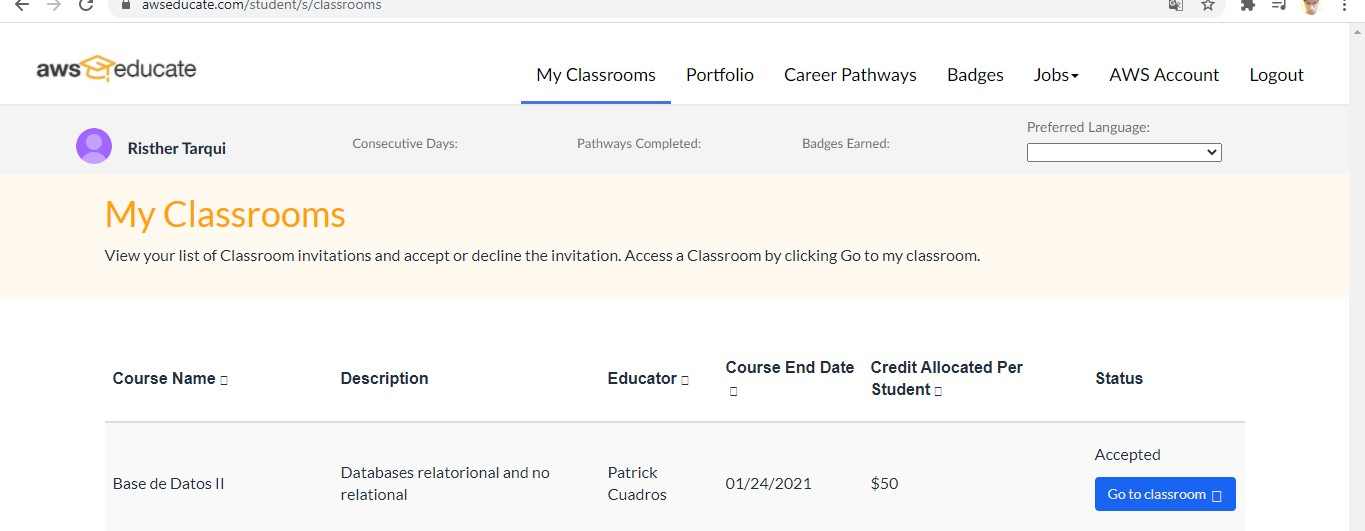
\includegraphics[width=14cm]{./img/1.1.jpg} 
		\end{center}
		
		\item Crear un bucket de Amazon S3
		En este laboratorio, debe especificar un bucket y una carpeta de Amazon S3 para almacenar los datos
		de salida de una consulta de Hive. En este laboratorio, se utiliza la ubicación predeterminada para los
		registros, pero también puede especificar una ubicación personalizada si lo desea. Debido a los
		requisitos de Hadoop, los nombres del bucket y de la carpeta que utilice con Amazon EMR tienen las
		siguientes limitaciones:
		• Deben incluir únicamente letras, números, puntos (.) y guiones (-).
		• No pueden terminar en números.
		Si ya tiene acceso a una carpeta que cumpla estos requisitos, puede utilizarla para este tutorial. La
		carpeta de salida debería estar vacía. Otro requisito que no hay que olvidar es que los nombres de los
		buckets deben ser únicos en todas las cuentas de AWS.
		Después de crear el bucket, elíjalo en la lista y, a continuación, elija Create folder (Crear carpeta),
		sustituya New folder (Carpeta nueva) por un nombre que cumpla los requisitos y, por último, elija Save
		(Guardar). El nombre del bucket y de la carpeta utilizado más adelante en el tutorial es s3://mybucket/
		MyHiveQueryResults. 
		\begin{center}
			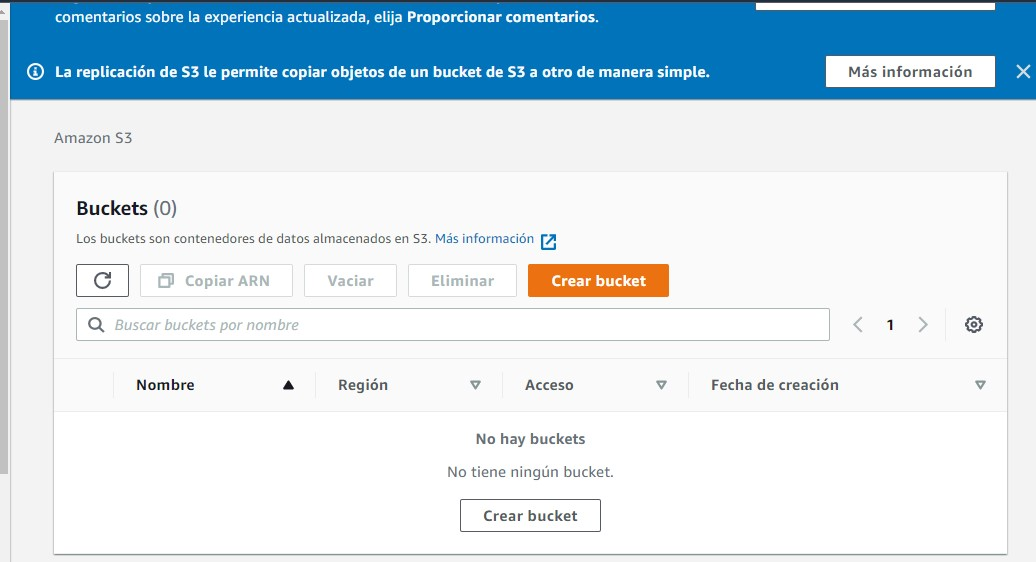
\includegraphics[width=14cm]{./img/1.2.1.jpg} 
		\end{center}
	\begin{center}
		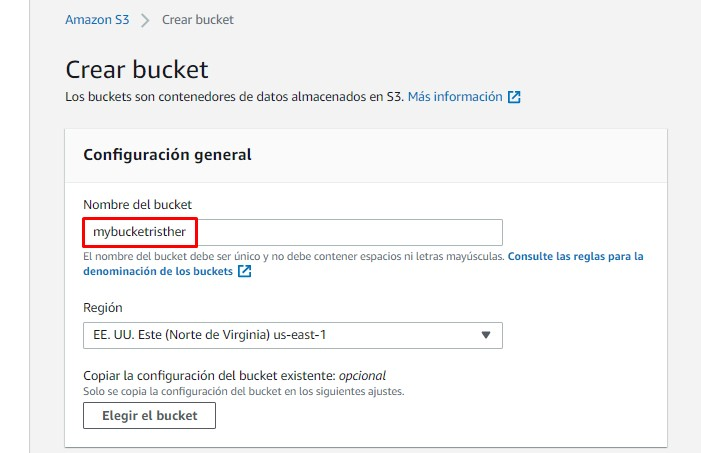
\includegraphics[width=14cm]{./img/1.2.2.jpg} 
	\end{center}
\begin{center}
	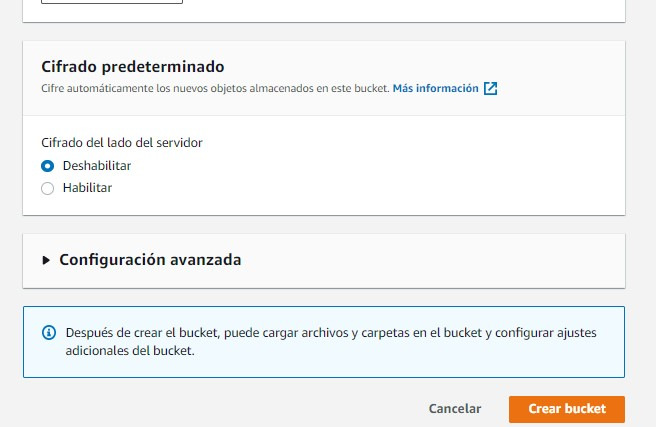
\includegraphics[width=14cm]{./img/1.2.3.jpg} 
\end{center}
	\begin{center}
	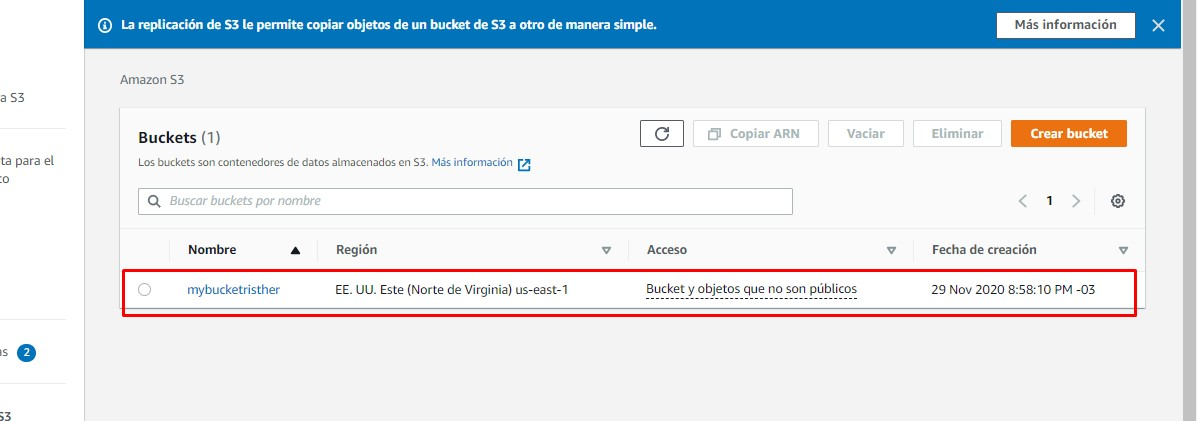
\includegraphics[width=14cm]{./img/1.2.4.jpg} 
\end{center}
\begin{center}
	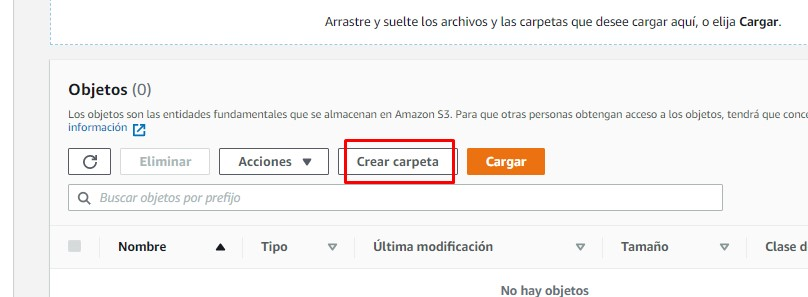
\includegraphics[width=14cm]{./img/1.2.5.jpg} 
\end{center}
\begin{center}
	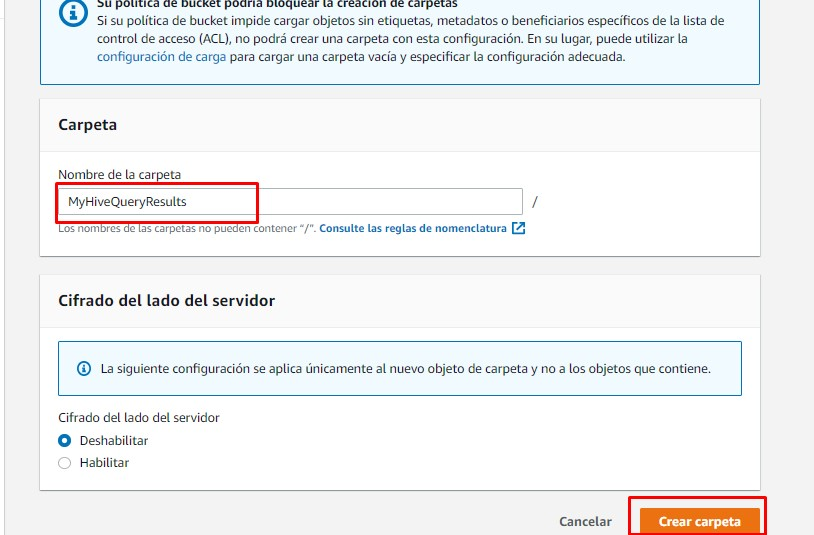
\includegraphics[width=14cm]{./img/1.2.6.jpg} 
\end{center}
		\item  Crear un par de claves de Amazon EC2
		Debe disponer de un par de claves de Amazon Elastic Compute Cloud (Amazon EC2) para conectarse a
		los nodos del clúster a través de un canal seguro mediante el protocolo Secure Shell (SSH). Puede omitir
		este paso si ya dispone del par de claves que desea utilizar. Si no dispone de un par de claves, siga uno
		de los procedimientos que se indican a continuación en función de su sistema operativo. 
			\begin{center}
			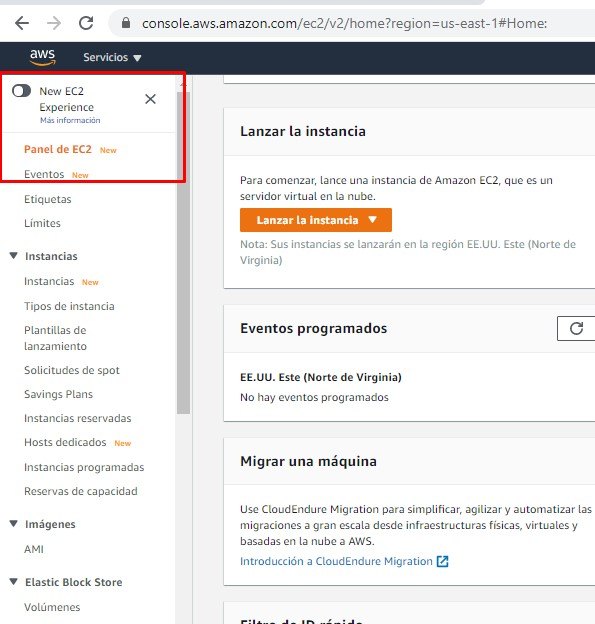
\includegraphics[width=14cm]{./img/1.3.1.jpg} 
		\end{center}
		\begin{center}
			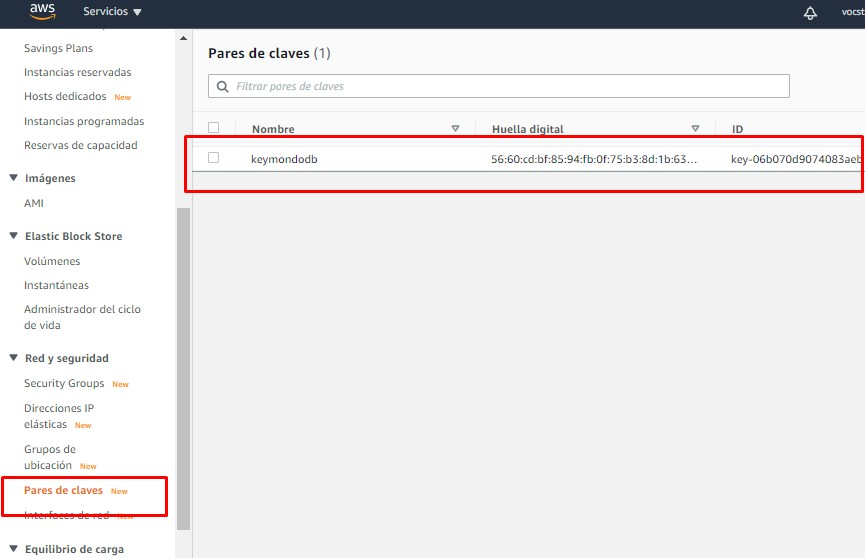
\includegraphics[width=14cm]{./img/1.3.2.jpg} 
		\end{center}
		
	
	
\subsection{Paso 2: Lanzar el clúster de Amazon EMR de ejemplo }
\item  En este paso, lanzará el clúster de ejemplo mediante las Quick Options (Opciones rápidas) de la consola de
Amazon EMR dejando la mayoría de las opciones con sus valores predeterminados.
También puede seleccionar Go to advanced options (Ir a las opciones avanzadas) para explorar las opciones
de configuración adicionales disponibles para un clúster.
	\begin{enumerate}
		
		\item Lanzar el clúster de ejemplo
		Para lanzar el clúster de Amazon EMR de ejemplo
	\\	a. Inicie sesión en la Consola de administración de AWS y abra la consola de Amazon EMR (https://
		console.aws.amazon.com/elasticmapreduce/).
		\begin{center}
			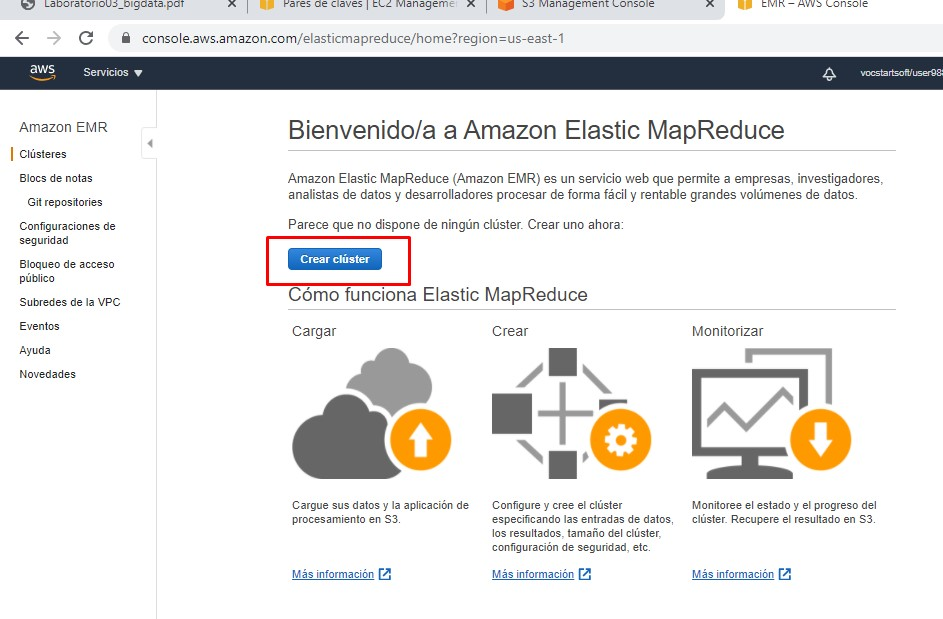
\includegraphics[width=14cm]{./img/2.1.jpg} 
		\end{center}
     \\	b. Elija Create cluster (Crear clúster).
     \begin{center}
     	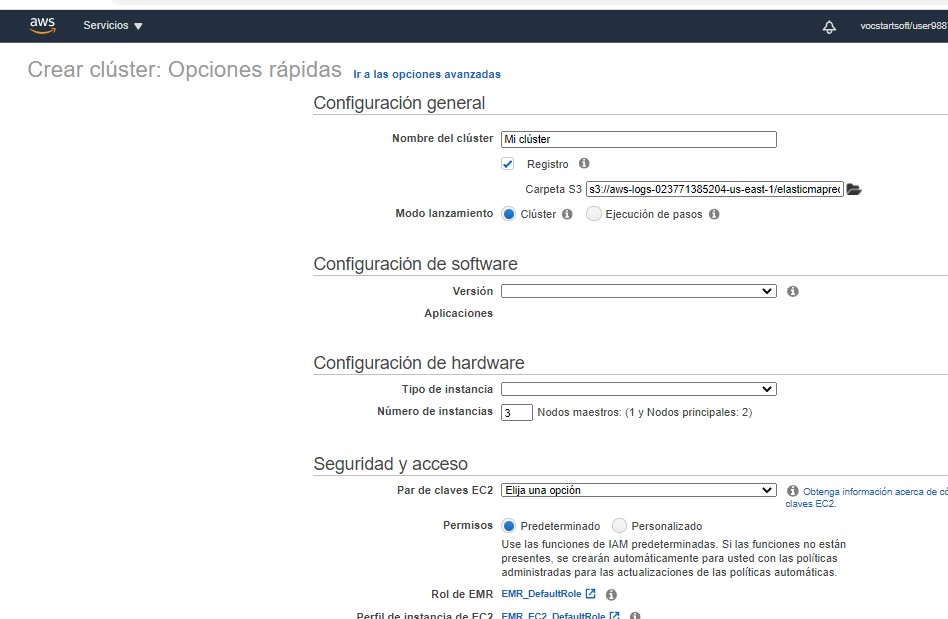
\includegraphics[width=14cm]{./img/2.2.jpg} 
     \end{center}
	\\	c. En la página Create Cluster - Quick Options (Crear clúster: opciones rápidas), acepte los valores
		predeterminados, excepto para los campos siguientes: 
		• Introduzca un Cluster name (Nombre del clúster) que le ayude a identificar el clúster, por
		ejemplo, Mi primer clúster de EMR.
		• En Security and access (Seguridad y acceso), elija el EC2 key pair (Par de claves EC2) que ha
		creado en Crear un par de claves de Amazon EC2.
		\begin{center}
			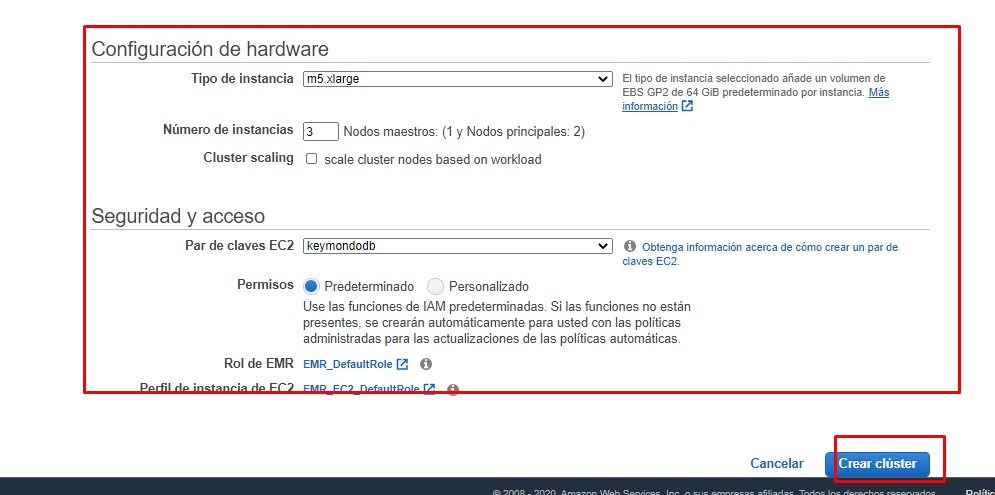
\includegraphics[width=14cm]{./img/2.3.jpg} 
		\end{center}
	\\	d. Elija Create cluster.
	
	\begin{center}
		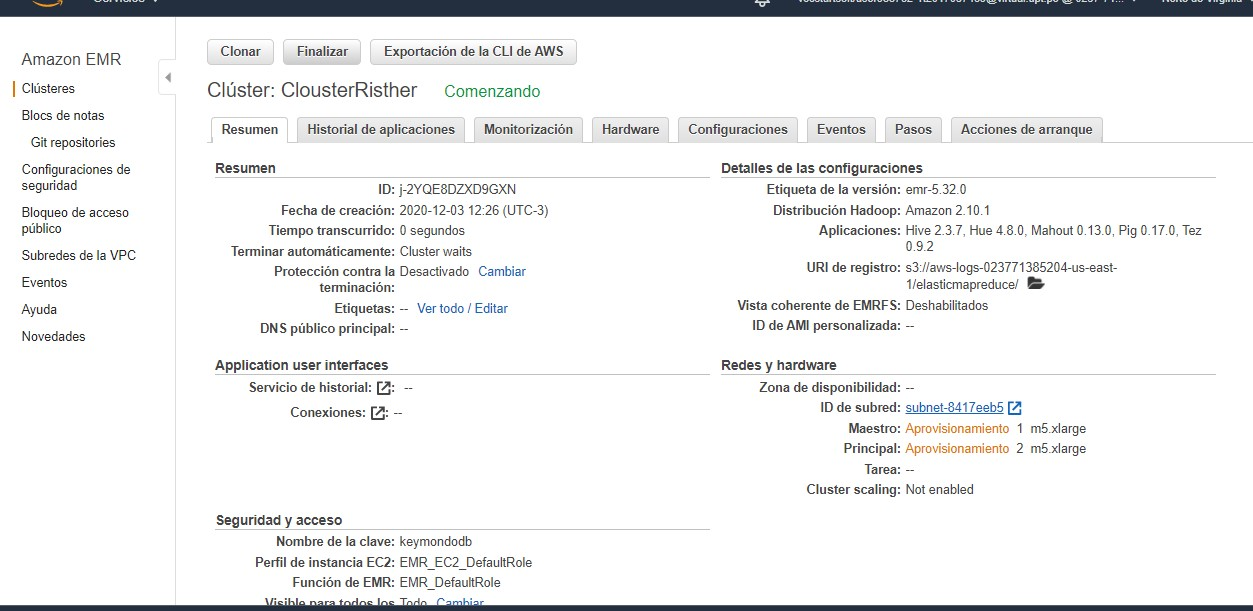
\includegraphics[width=14cm]{./img/2.4.jpg} 
	\end{center}
\end{enumerate}
	\subsection{Paso 3: Permitir las conexiones SSH con el clúster desde el cliente }
		\item	Los grupos de seguridad funcionan como firewalls virtuales para controlar el tráfico entrante y saliente del
		clúster. Al crear el primer clúster, Amazon EMR crea el grupo de seguridad administrado por Amazon EMR
		por defecto asociado a la instancia principal, ElasticMapReduce-master y el grupo de seguridad asociado a
		los nodos principal y de tareas, ElasticMapReduce-slave.
		Para restringir el acceso mediante SSH para el grupo de seguridad ElasticMapReduce-master Se debe haber
		iniciado sesión primero en AWS como usuario raíz o como principal de IAM con permiso para administrar
		grupos de seguridad para la VPC en la que se encuentra el clúster. Para más información, consulte Cambio
		de los permisos de un usuario de IAM y el Ejemplo de política que permite administrar grupos de seguridad
		de EC2 en la Guía del usuario de IAM.

	\begin{enumerate}
		
		\item Abra la consola de Amazon EMR en https://console.aws.amazon.com/elasticmapreduce/
	\begin{center}
		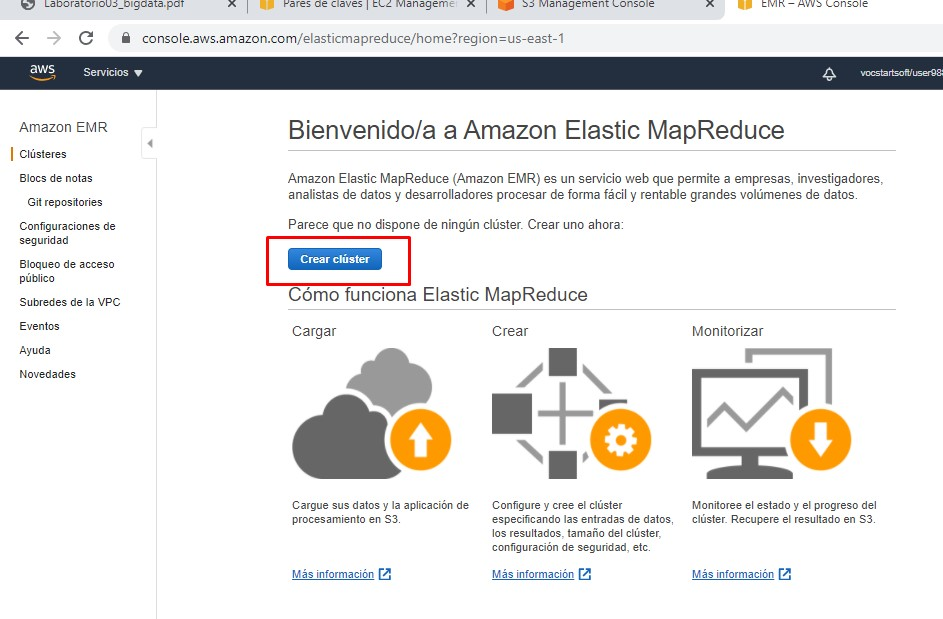
\includegraphics[width=14cm]{./img/3.1.jpg} 
	\end{center}
		\item Seleccione Clusters (Clústeres). 

		
		\item
		 Elija el Name (Nombre) del clúster. 
		
	
		\item	En Security and access (Seguridad y acceso), elija el enlace Security groups for Master (Grupos de
			seguridad para principal).
			\begin{center}
				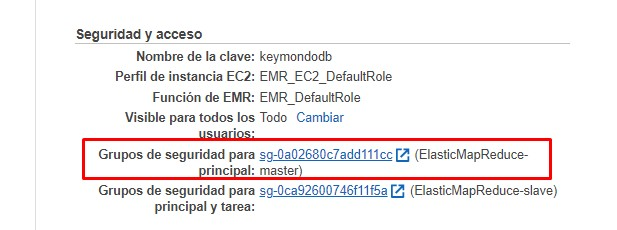
\includegraphics[width=14cm]{./img/3.4.jpg} 
			\end{center}
		\item Elija ElasticMapReduce-master en la lista. 
		\begin{center}
			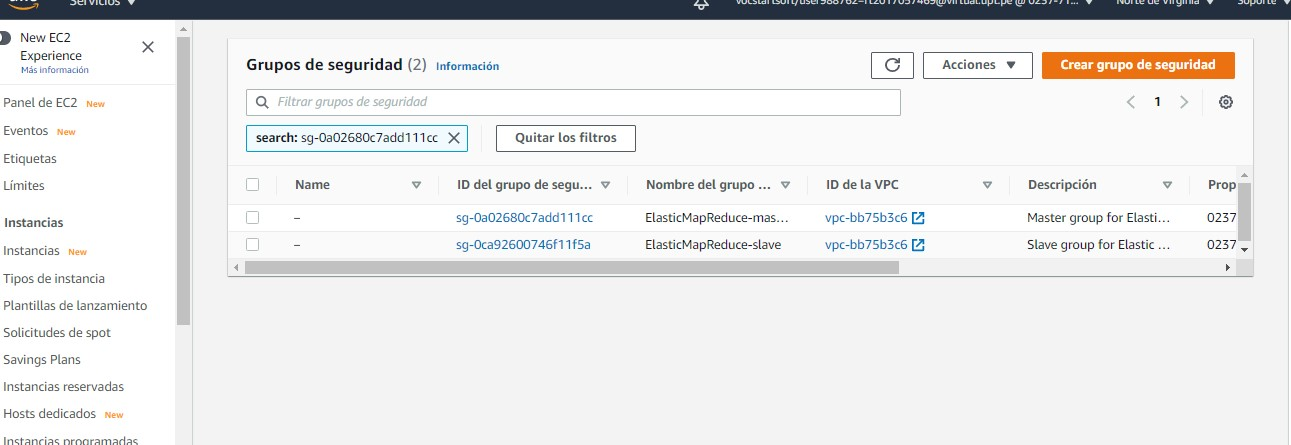
\includegraphics[width=14cm]{./img/3.5.jpg} 
		\end{center}
		\item Elija Inbound (Entrada), Edit (Editar). 
		\begin{center}
			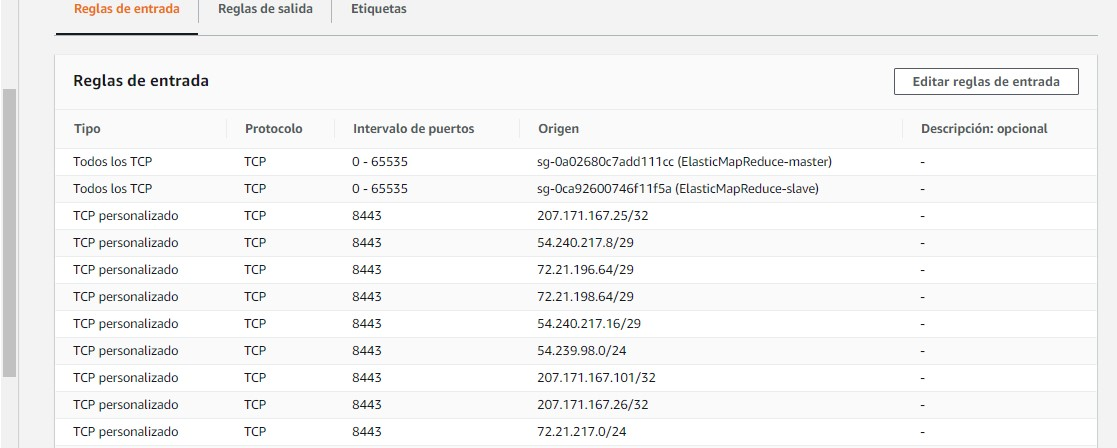
\includegraphics[width=14cm]{./img/3.6.jpg} 
		\end{center}
		\item Compruebe si hay una regla de entrada que permite el acceso público con la siguiente configuración. Si
		existe, elija Delete (Eliminar) para eliminarla.
		• Type (Tipo) SSH
		• Port (Puerto) 22
		• Source (Fuente) Personalizada 0.0.0.0/0 
		\item Desplácese a la parte inferior de la lista y elija Add Rule (Añadir regla). 
		\begin{center}
			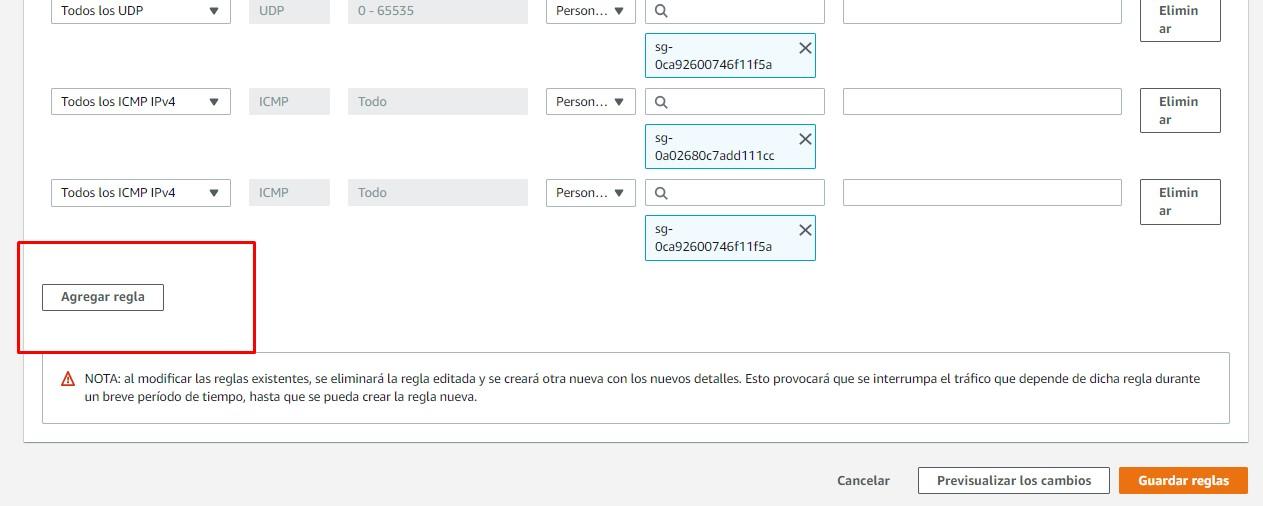
\includegraphics[width=14cm]{./img/3.8.jpg} 
		\end{center}
		\item En Type (Tipo), seleccione SSH. Esto introduce automáticamente TCP para Protocol (Protocolo) y 22
		para Port Range (Rango de puertos). 
		\item Como origen, seleccione My IP (Mi IP). Esto añade automáticamente la dirección IP del equipo cliente
		como la dirección de origen. También puede añadir un rango de direcciones IP de clientes de confianza
		Custom (Personalizadas) y elegir Add rule (Añadir regla) para crear reglas adicionales para otros
		clientes. Muchos entornos de red asignan dinámicamente direcciones IP, por lo que es posible que 
		necesite editar periódicamente las reglas de grupos de seguridad para actualizar las direcciones IP de
		los clientes de confianza. 
		\begin{center}
			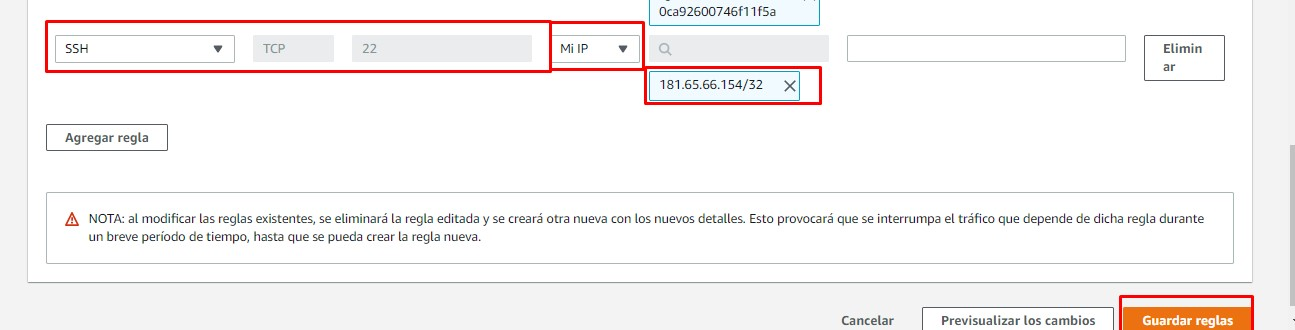
\includegraphics[width=14cm]{./img/3.10.jpg} 
		\end{center}
		\item Elija Save (Guardar).
		\begin{center}
			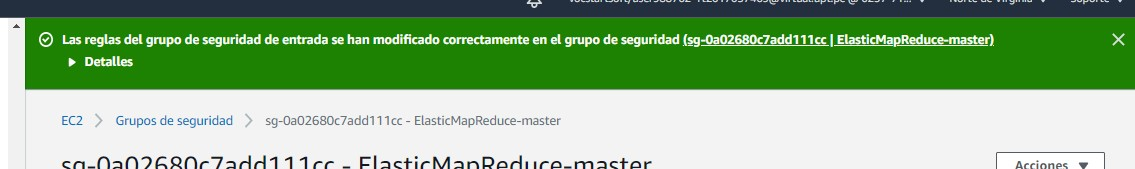
\includegraphics[width=14cm]{./img/3.11.jpg} 
		\end{center}

\end{enumerate}	
	\subsection{Paso 4: Procesar los datos ejecutando el script de Hive como paso
}
\begin{enumerate}
	\item	 Abra la consola de Amazon EMR en https://console.aws.amazon.com/elasticmapreduce/
	\item En Cluster List (Lista de clústeres), seleccione el nombre del clúster. Asegúrese de que el clúster está en
	el estado Waiting (Esperando). 
	\item	 Elija Steps (Pasos) y, a continuación Add step (Añadir paso). 
	\begin{center}
		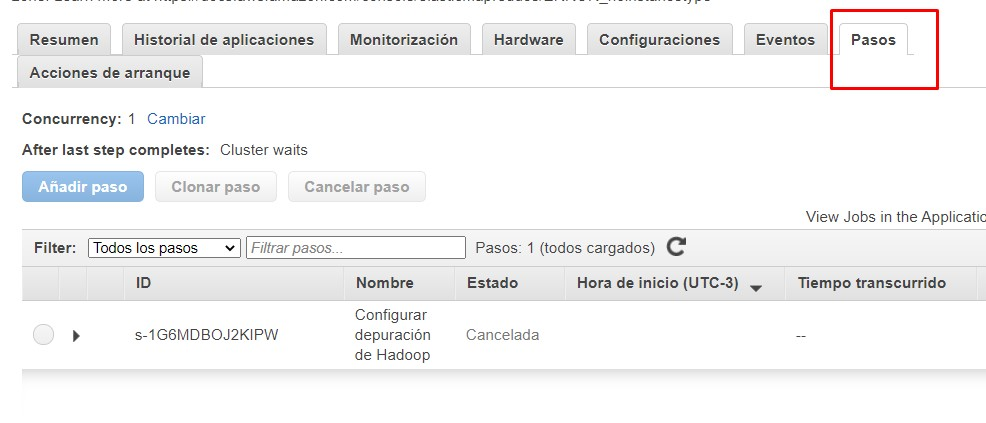
\includegraphics[width=14cm]{./img/4.3.jpg} 
	\end{center}
	\item  Configure el paso de acuerdo con las directrices siguientes:
	• En Step type (Tipo de paso), elija Hive program (Programa de Hive).
	• En Name (Nombre), puede dejar el valor predeterminado o escribir un nombre nuevo. Si tiene
	muchos pasos en un clúster, el nombre le ayuda a realizar un seguimiento de ellos.
	• En Script S3 location (Ubicación en S3 del script), escriba
	s3://region.elasticmapreduce.samples/cloudfront/code/Hive_CloudFront.q. Sustituya region por el
	identificador de la región. Por ejemplo, s3://uswest2.elasticmapreduce.samples/cloudfront/code/Hive_CloudFront.q si está trabajando en la región de
	Oregon (Oregón).
	• En Input S3 location (Ubicación en S3 de la entrada), escriba s3://region.elasticmapreduce.samples
	Sustituya region por el identificador de la región.
	• En Output S3 location (Ubicación en S3 de la salida), escriba o busque el bucket output que creó en
	Crear un bucket de Amazon S3 (p. 12).
	• En Action on failure (Acción sobre el error), acepte la opción predeterminada Continue (Continuar).
	Esto especifica que si se produce un error en el paso, el clúster sigue ejecutándose y procesa los pasos
	siguientes. La opción Cancel and wait (Cancelar y esperar) especifica que los pasos con error deben
	cancelarse y que los pasos siguientes no se deben ejecutar, pero que el clúster debe seguir
	ejecutándose. La opción Terminate cluster (Terminar clúster) especifica que el clúster debe terminarse
	si el paso genera un error. 
	\begin{center}
		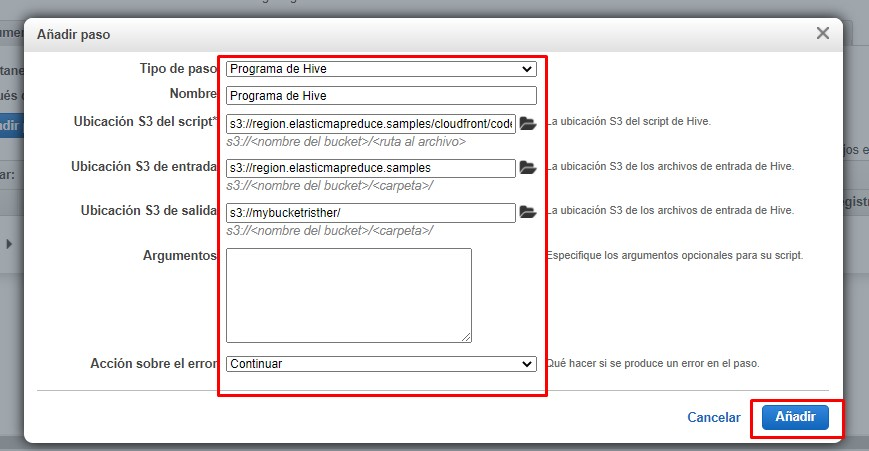
\includegraphics[width=14cm]{./img/4.4.jpg} 
	\end{center}
	\item	Elija Add (Añadir). El paso aparece en la consola con el estado Pending (Pendiente). 
	\begin{center}
		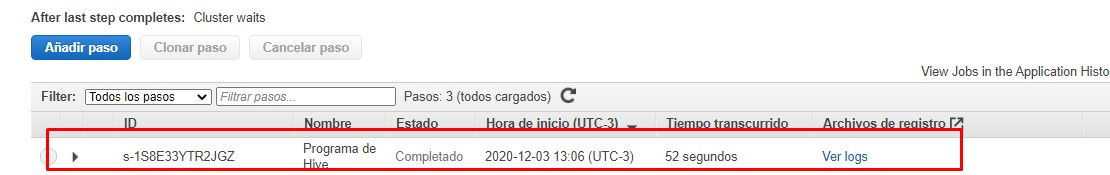
\includegraphics[width=14cm]{./img/4.5.jpg} 
	\end{center}
	\item  El estado del paso cambia de Pending (Pendiente) a Running (En ejecución) y a Completed
	(Completado) a medida que se ejecuta. Para actualizar el estado, elija el icono de actualización situado
	a la derecha de Filter (Filtro). El script tarda aproximadamente un minuto en ejecutarse. 
	
	\\ 1. Abra la consola de Amazon S3 en https://console.aws.amazon.com/s3/.
	\begin{center}
		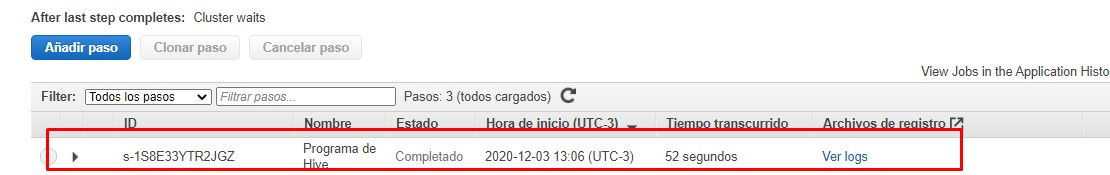
\includegraphics[width=14cm]{./img/4.5.jpg} 
	\end{center}
\\ 	2. Elija el Bucket name (Nombre del bucket) y, a continuación, elija la carpeta que ha configurado
	anteriormente. Por ejemplo, mybucket y luego MyHiveQueryResults.
	\\ 3. La consulta escribe los resultados en una carpeta ubicada en la carpeta de salida denominada
	os_requests. Elija esa carpeta. Debería haber un único archivo denominado 000000_0 en dicha
	carpeta. Se trata de un archivo de texto que contiene los resultados de la consulta de Hive.
	\\ 4. Elija el archivo y, a continuación, elija Download (Descargar) para guardarlo localmente.
	\\ 5. Utilice el editor de texto que prefiera para abrir el archivo. El archivo de salida muestra el número
	de solicitudes de acceso ordenadas por sistema operativo. El siguiente ejemplo muestra la salida en
	WordPad:
	\begin{center}
		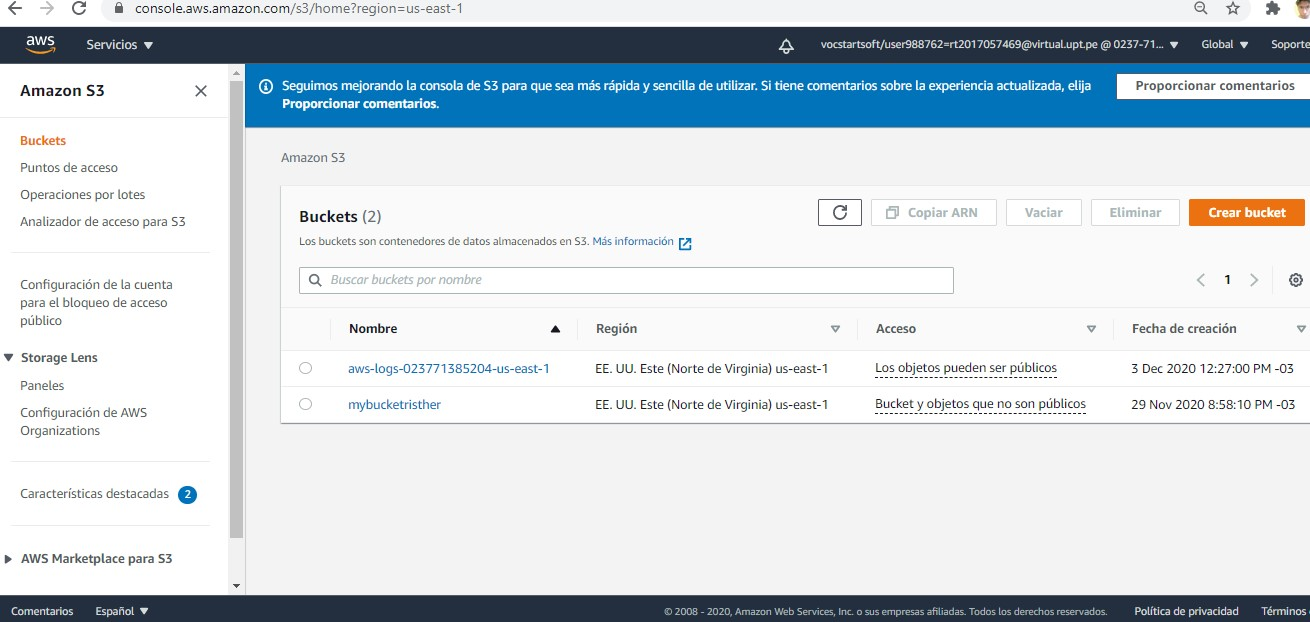
\includegraphics[width=14cm]{./img/4.6.1.jpg} 
	\end{center}
    \begin{center}
    	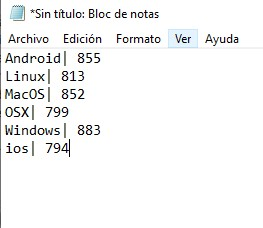
\includegraphics[width=14cm]{./img/4.6.jpg} 
    \end{center}
	\subsection{Paso 5: Terminar el clúster y eliminar el bucket 
}

\item Es conveniente que termine el clúster y elimine el bucket de Amazon S3 para evitar cargos adicionales. Al
terminar el clúster, terminan las instancias Amazon EC2 asociadas y se detiene la acumulación de cargos de
Amazon EMR. Amazon EMR conserva la información de metadatos sobre los clústeres completados para su
referencia, gratuitamente, durante dos meses. La consola no proporciona una forma de eliminar clústeres
terminados, por lo que no se pueden ver en la consola. Los clústeres terminados se eliminan del clúster al
eliminar los metadatos. 	

	\begin{enumerate}
	
	\item . Abra la consola de Amazon EMR en https://console.aws.amazon.com/elasticmapreduce/. 
	\begin{center}
		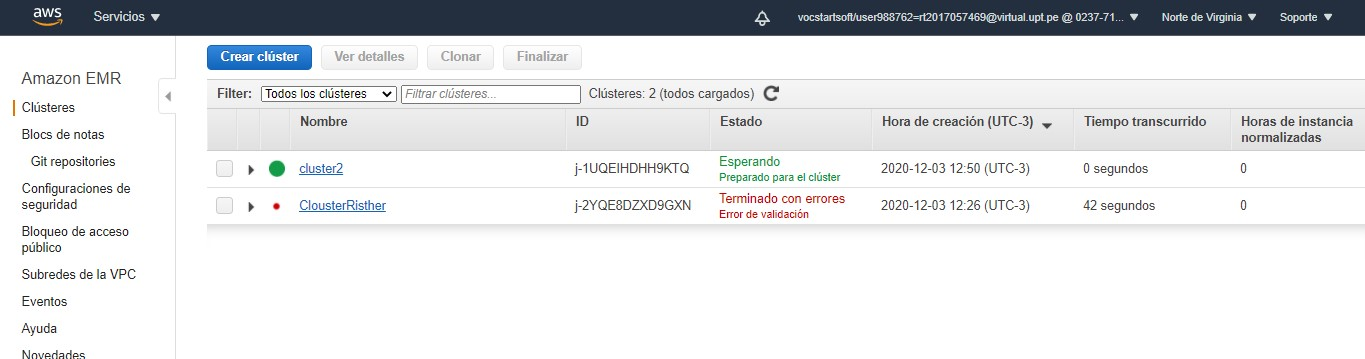
\includegraphics[width=14cm]{./img/5.1.jpg} 
	\end{center}
	\item Elija Clusters (Clústeres), elija el clúster y, a continuación, Terminate (Terminar).
	Los clústeres suelen crearse con la protección de terminación activada, lo que ayuda a evitar que se
	cierren de forma accidental. Si ha seguido el tutorial al pie de la letra, la protección de terminación
	debería estar desactivada. Si la protección de terminación está activada, se le pedirá que cambie esta
	opción como medida de precaución antes de terminar el clúster. Elija Change (Cambiar), Off
	(Desactivada). 
	\begin{center}
		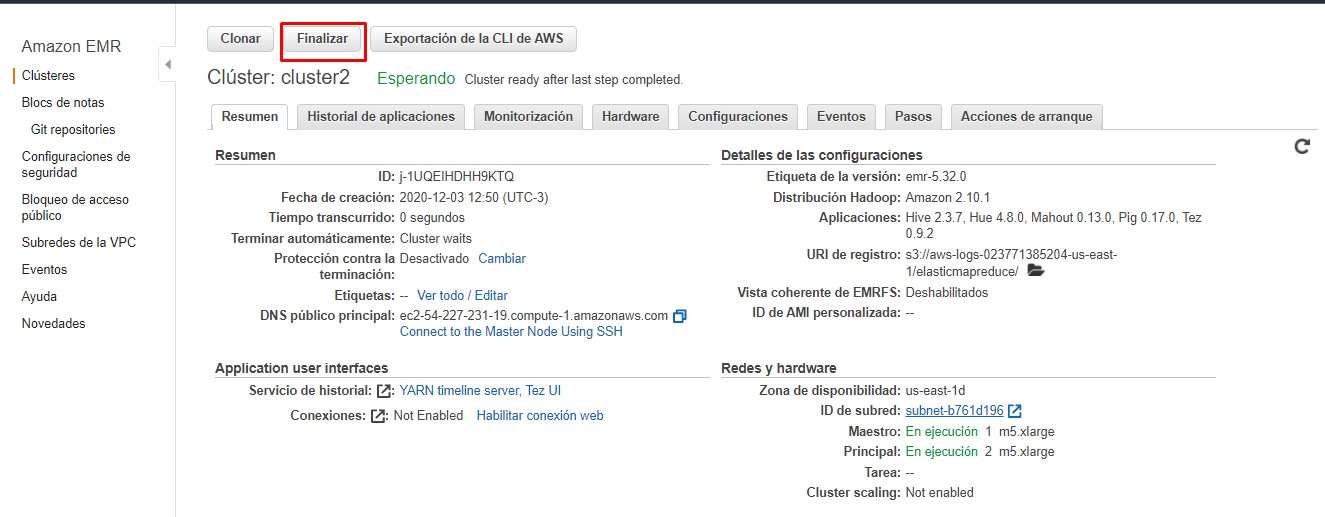
\includegraphics[width=14cm]{./img/5.2.jpg} 
	\end{center}
	\item Para eliminar el bucket de salida
 \\	1. Abra la consola de Amazon S3 en https://console.aws.amazon.com/s3/
\\	2. Elija el bucket en la lista, de forma que toda la fila del bucket esté seleccionada. 3. Elija eliminar el
	bucket, escriba el nombre de este y, a continuación, haga clic en Confirm (Confirmar).
	Para obtener más información sobre la eliminación de carpetas y buckets, vaya a ¿Cómo elimino un
	bucket de S3? en la Guía de introducción a Amazon Simple Storage Service.

	\begin{center}
		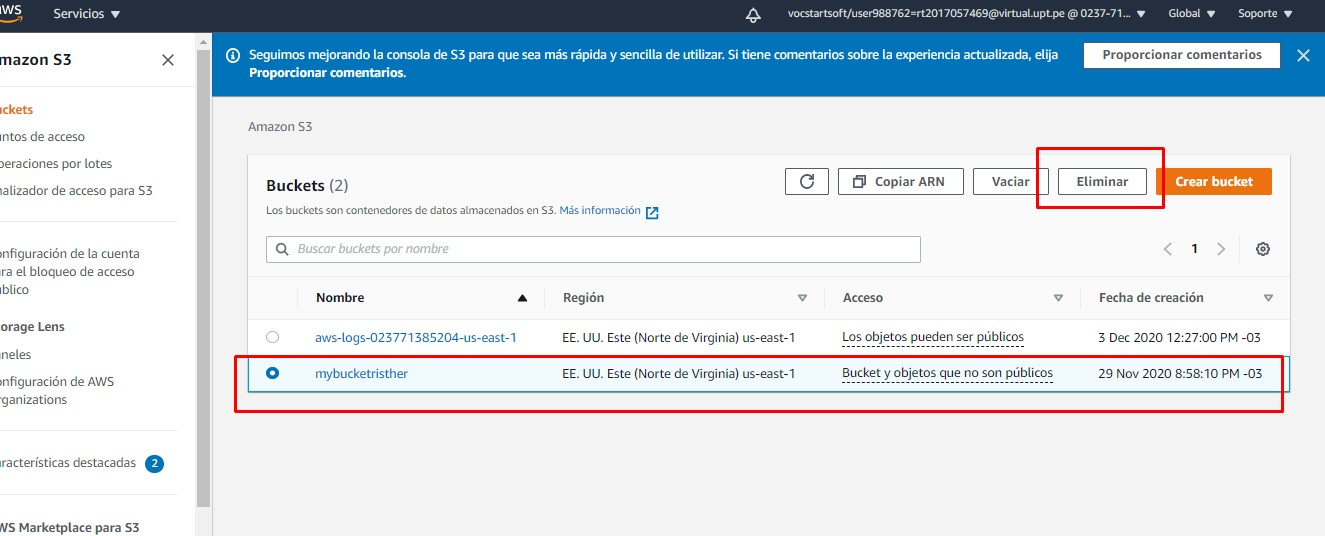
\includegraphics[width=14cm]{./img/5.2.1.jpg} 
	\end{center}
\end{enumerate}	
		
	\section{CONCLUSIONES}
	\begin{itemize}
			\item Se creo un bucket y un par de keys para la creacion de cluster, dentro del cluster editamos la reglas de entrada para conexion mediante ssh.Finalmente creamos un paso con el cluster en la carpeta de bucket que se creo al incio.
			\end{itemize}
		
		
	\end{document}